% !TEX root = ../main.tex
\section{Method}
\label{sec:method}

Given a training set $\mathcal{D} = \{(x_i, y_i)\}_{i=1}^{n}$, a model $h_\theta$ is fitted by minimizing the empirical risk
\begin{equation}
  \hat{\theta} \in \arg\min_{\theta} \frac{1}{n} \sum_{i=1}^{n} \ell\big(h_\theta(x_i), y_i\big).
  \label{eq:erm}
\end{equation}

Figure~\ref{fig:pipeline} summarizes the writing workflow.

\begin{figure}[ht]
  \centering
  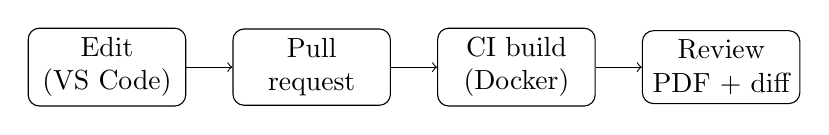
\begin{tikzpicture}[node distance=2.6cm, every node/.style={draw, rounded corners, minimum width=2cm, minimum height=0.8cm, align=center}]
    \node (edit) {Edit\\(VS Code)};
    \node (pr) [right of=edit] {Pull\\request};
    \node (ci) [right of=pr] {CI build\\(Docker)};
    \node (review) [right of=ci] {Review\\PDF + diff};
    \draw[->] (edit) -- (pr);
    \draw[->] (pr) -- (ci);
    \draw[->] (ci) -- (review);
  \end{tikzpicture}
  \caption{Writing workflow.}
  \label{fig:pipeline}
\end{figure}
